\section{Reinforcement Learning Framework}\raggedbottom 
The main components of the reinforcement learning framework are the \textit{agent} and the \textit{environment}.

An agent interacts with the \textit{environment} over time, by taking in the environment state, which is usually denoted as $s$ or $x$. Within this work, $s$ will be used as notation for the state.
The agent evaluates the state and decides on an \textit{action} (denoted as $a$), based on the current state. 

A problem distinct to reinforcement learning is the one of exploration and exploitation. In order to learn the best behavior, the \textit{agent} needs to make sure to explore the \textit{environment}. Insufficient exploration can lead to suboptimal policies since a path that leads to a high reward might not be found. 

Whenever the agent interacts with the environment, it receives a \textit{reward} and the next state in return.
Depending on whether the environment is terminal or not, an additional value denoting if the environment has terminated is received. 
The Atari games considered within this work terminate if the player either wins or loses the game.

\begin{figure}
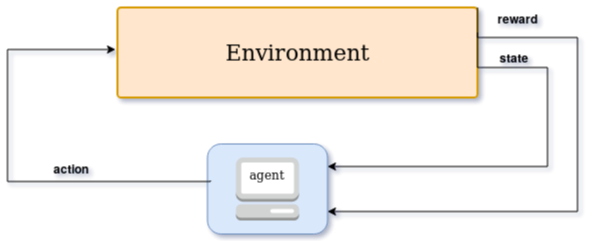
\includegraphics[width=90mm]{bilder/RLFramework.png}
\caption{Agent interacting with the environment}
\end{figure}


\subsection{Elements of Reinforcement Learning}
\citet{Sut98} name the following 4 other core elements of the reinforcement learning framework.

\textbf{Policy}

The behavior of the agent at any given time $t$ is determined by the \textit{policy}. A policy $\pi$ can roughly be described as a mapping of states to an action or a distribution over actions. 
We denote the probability of an action $a$ being taken at state $s$ and time $t$ under a policy $\pi$ as
\begin{equation}
P_\pi( a \mid s_t) = \pi(a \mid s_t) . 
\end{equation}
Within this work, the policy is always stochastic and the probability distribution over actions is denoted as $\pi (\bullet \mid s)$.
\pagebreak

\textbf{Reward Signal}

The problem posed by an environment is defined through the reward function. 

The goal of the learning agent is to receive the maximum accumulated future reward at any given time. One of the most important features of reinforcement learning is the fact, that rewards are often significantly delayed. 

Connecting the delayed reward with the actions that caused it is a key task of reinforcement learning.
A great example for this problem is the game Pong. The reward is caused by successfully playing the ball, however only many frames later, after the opponent missed the ball, the reward is received.

Games like chess pose an even bigger problem since every move can play an important role in winning the game. Good opening moves can strongly impact if the game is lost or won 100 moves later.

The reward received by an agent at timestep $t$ will be denoted as $r_t$.

\textbf{Value Function}

The state-value represents the sum of the future rewards and indicates the long-term desirability of a state.

The value of a state at timestep $t$ under a policy $\pi$ is given through the expectancy of the \textit{return} $R_t$ , which is the possible accumulated future reward denoted as $V(s)$ and given by:

\begin{equation}
{
V^\pi (s) = E_\pi \{R_t \mid s_t = s\} = E_\pi \left\{ \sum_{k=0}^\infty \gamma^k r_{t+k+1} \mid s_t = s \right\}
}
\end{equation}

where $\gamma$ denotes the discount factor. By discounting rewards, we can decide how important short-term rewards are in comparison to rewards in the distant future.

In accordance with this, we define the state-action value $Q(s,a)$, which is the expected return, if the action $a$ is taken at state $s$.

\begin{equation}
{
Q^\pi (s,a) = E_\pi \{R_t \mid s_t = s, a_t = a\} = E_\pi \left\{ \sum_{k=0}^\infty \gamma^k r_{t+k+1} \mid s_t = s, a_t = a \right\}
}
\end{equation}

Additionally we define the advantage $A^\pi(s,a)$ for an \textit{action} $a$ at state $s$.

\begin{equation}
A^\pi(s,a) = Q^\pi(s,a)-V^\pi(s)
\label{adv}
\end{equation}

The advantage of an action given a state denotes how much better this action is, compared to the average action.

\textbf{Environment Model}

In order to solve a problem, a model of the environment can be learned and used for planning. A model can be used to predict future states and rewards before they happen.
Model-based and model-free reinforcement learning methods, which explicitly learn by trial and error both play an important role in reinforcement learning.

Within this thesis, we will only look at model-free methods. Rather than learning a model, the agent learns directly through trajectories sampled from the environment.

\pagebreak

\subsection{Markov Decision Process} 

We can describe the sequential decision-making process of the \textit{agent} more formally as a Markov decision process (MDP).

The sequential decision-making process is given by a sequence of states, actions and rewards:

$s_0, a_0, r_0, s_1, a_1, r_1, s_2, a_2, r_2, \dots, s_t,a_t,r_t, s_{t+1}$

Such sequences are called \textit{trajectories}.

Within this thesis, we assume the environment to be finite.

A state is called \textit{Markov} or said to have \textit{Markov property} if it only depends on its predecessor rather than the whole history.
\begin{equation}
P(s_{t+1} = s', r_{t+1} = r' \mid s_t, a_t, r_t, s_{t-1}, \dots ,r_1,a_0,s_0) = P(s_{t+1} = s', r_{t+1} = r' \mid s_t,a_t)
\end{equation}

A finite discounted Markov decision process $MDP(S,A,P_a,R_a,\gamma)$ contains a finite set of states $S$, 
a finite set of actions $A$,
the transition probablity to end up in state $s'$ if action $a$ is taken in state $s$ : 
\begin{equation}
P^a_{s s'} = Pr(s_{t+1} = s' \mid s_t = s, a_t = a)
\end{equation}

the reward function $R^a_{s s'}$,
and the discount factor $\gamma  \in [0,1)$.

\subsection{Deep Reinforcement Learning}
In contrast to directly mapping an input to an output value, deep learning algorithms contain so-called \textit{hidden layers}.


Usually, a transformation or activation function is applied to the input of each hidden layer. Rectified linear units (ReLU), the tanh or the sigmoid function can be named as popular activation functions.
After feeding an input into the network and calculating an error value, the weights are adjusted through backpropagation.

Convolutional neural networks (CNN) were inspired by visual neuroscience and are great tools to process image data. CNNs mainly consist of convolutional layers, pooling layers, and fully connected layers.
Other relevant approaches are recurrent neural networks (RNN) or long-short-term memory networks (LSTM). Both mimic functions of a memory and have started to play bigger roles within the field of deep reinforcement learning recently.

Combining deep learning methods with reinforcement learning methods was a major breakthrough, enabling reinforcement learning methods to be successfully applied to complex problems like those posed by the Atari 2600 console \citep{deeprlLi}.

This thesis works with CNNs, consisting of convolutional layers, dense layers, and ReLU activation functions.
\pagebreak
Convolutional layers are used to extract features from image data. By moving filters over the image and calculating the weighted sum of the filter and the respective parts of the images the output is calculated. 

The outputs are weighted sums of parts from the original image.
The \textit{stride} denotes how much a filter is shifted before being applied to the image again. Multiple filters are used to receive many different features.

\begin{figure}
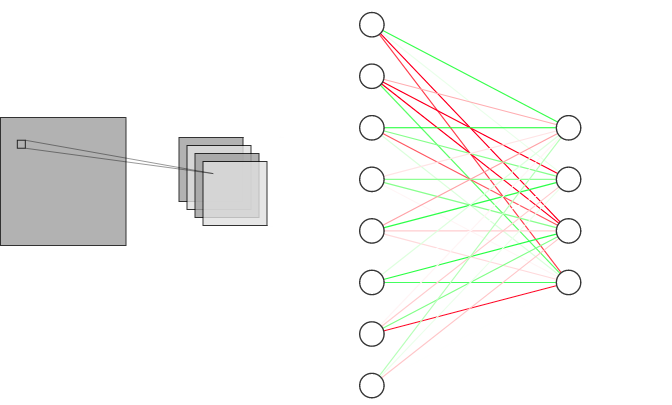
\includegraphics[scale=0.5]{bilder/deeplayers.png}
\caption{A convolutional (left) and fully connected (right) layer.
}
\label{networks}
\end{figure}

Fully Connected Layers are used to weight the input and map it to the output space. 

Each 'Neuron' or element in the output layer, holds a weighted sum of every input element (Figure \ref{networks}).

The ReLU function changes all negative values to 0, while positive values remain untouched:

\begin{equation}
ReLU (x) = 
\begin{cases}
x & \text{if x >0} \\
0 & else
\end{cases}
\end{equation}


\pagebreak